\documentclass[11pt]{article}
\usepackage[utf8]{inputenc}
\usepackage[T1]{fontenc}
\usepackage{graphicx}
\usepackage[export]{adjustbox}
\graphicspath{ {./images/} }
\usepackage{amsmath}
\usepackage{amsfonts}
\usepackage{amssymb}
\usepackage[version=4]{mhchem}
\usepackage{stmaryrd}

\begin{document}
Real Estate Style Boxes

The first part of this session detailed the use of NCREIF real estate styles to differentiate real estate properties and portfolios by their risks and returns. These categories can be used to create and use real estate style boxes.

Real estate style boxes use two categorizations of real estate to generate a box or matrix that can be used to characterize properties or portfolios. The next exhibit illustrates style boxes for traditional investments. In the case of the equity style box on the left, the box has equity style on the horizontal axis (e.g., value versus growth) and capitalization size on the vertical axis. In traditional bond analysis, duration is usually on the horizontal axis, with credit quality on the vertical axis.\\
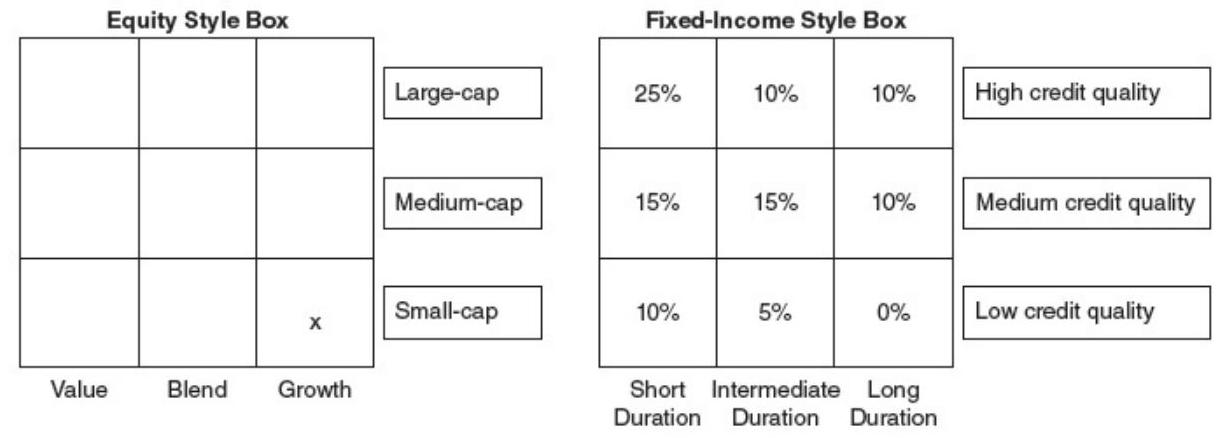
\includegraphics[max width=\textwidth, center]{2024_04_11_515942530f610ac594f4g-2(1)}

\section*{Equity and Fixed-Income Style Boxes}
Style boxes are applied to individual assets, managers, or portfolios. For a style box of an individual stock or bond, the box contains an X in the square most descriptive of the asset. Similarly, managers can be identified with an X in a style box to denote their primary focus. The equity style box in Equity and Fixed-Income Style Boxes illustrates the use of an $\mathrm{X}$ in a single square to denote the primary characteristic of a hypothetical small-cap growth fund. Portfolios and funds are often identified with percentages in each square denoting how much of the fund's or portfolio's holdings are invested in assets of each location. The fixed-income box on the right of the above exhibit illustrates the use of percentages in each of the nine squares.

The next exhibit illustrates real estate style boxes. There is no uniform standard for style boxes in the real estate industry. Clearly, for private commercial equity, the styles of NCREIF are prime candidates for the horizontal axis. Primary, secondary, and tertiary real estate markets are potentially useful for the vertical axis. The left side of next exhibit illustrates a potential style box and hypothetical allocations. In this illustration, a real estate style box serves as a method of better understanding the top-down allocations of a real estate portfolio. A real estate style box can also be used to denote the location of a single manager or a single property by placing an $\mathrm{X}$ in the relevant square.

\begin{center}
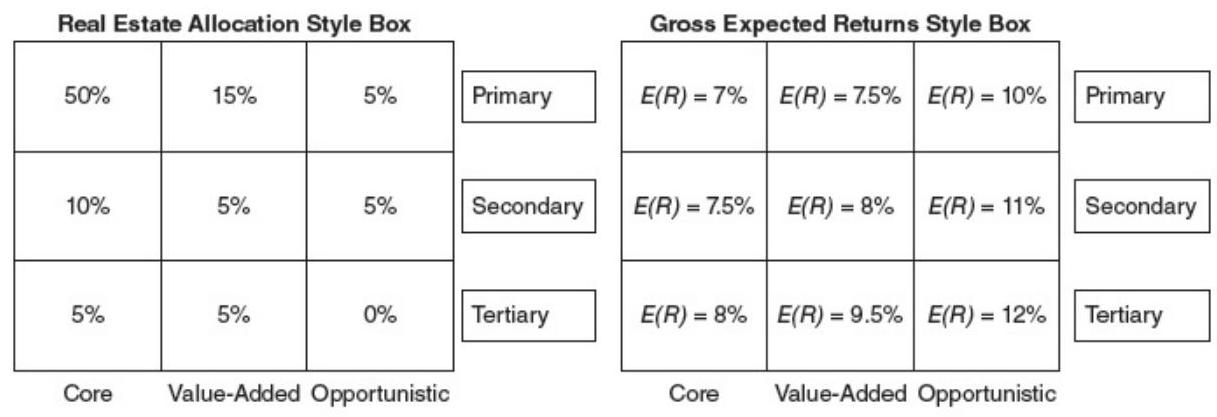
\includegraphics[max width=\textwidth]{2024_04_11_515942530f610ac594f4g-2}
\end{center}

Real Estate Style Boxes


\end{document}